%------------------------
% CV
% Author : Kevin Rojas
% Github : https://github.com/krojasalfaro7
%------------------------

%BASE
%------------------------
% Resume Template
% Author : Anubhav Singh
% Github : https://github.com/xprilion
% License : MIT
%------------------------

\documentclass[a4paper,20pt]{article}

\usepackage{latexsym}
\usepackage[empty]{fullpage}
\usepackage{titlesec}
\usepackage{marvosym}
\usepackage[usenames,dvipsnames]{color}
\usepackage{verbatim}
\usepackage{enumitem}
\usepackage[pdftex]{hyperref}
\usepackage{fancyhdr}
\usepackage{graphicx} % Para insertar imagenes
\usepackage{array} % Para el manejo de tablas con tamanio
\usepackage[usenames]{color} % Para el color de las URL

\pagestyle{fancy}
\fancyhf{} % clear all header and footer fields
\fancyfoot{}
\renewcommand{\headrulewidth}{0pt}
\renewcommand{\footrulewidth}{0pt}

% Adjust margins
\addtolength{\oddsidemargin}{-0.530in}
\addtolength{\evensidemargin}{-0.375in}
\addtolength{\textwidth}{1in}
\addtolength{\topmargin}{-.45in}
\addtolength{\textheight}{1in}

\urlstyle{rm}

\raggedbottom
\raggedright
\setlength{\tabcolsep}{0in}
%\moderncvstyle{casual}   

% Sections formatting
%\titleformat{\section}{
%  \vspace{-5pt}\scshape\raggedright\large
%}{}{0em}{}[\color{black} \vspace{-2pt}]

% Section titles
%\titleformat{\section}{
%    \scshape\raggedright\Large\color{Blue}}{}{0em}{}[\color{Blue}\titlerule
%    \vspace{-\smallskipamount}]

\titleformat{\section}{
  \vspace{-10pt}\scshape\raggedright\large
}{}{0em}{}[\color{black}\titlerule \vspace{-6pt}]

%-------------------------
% Custom commands
\newcommand{\resumeItem}[2]{
  \item\small{
    \textbf{#1}{: #2 \vspace{-2pt}}
  }
}

\newcommand{\resumeItemWithoutTitle}[1]{
  \item\small{
    {\vspace{-2pt}}
  }
}

\newcommand{\resumeSubheading}[4]{
  \vspace{-1pt}\item
    \begin{tabular*}{0.97\textwidth}{l@{\extracolsep{\fill}}r}
      \textbf{#1} & #2 \\
      \textit{#3} & \textit{#4} \\
    \end{tabular*}\vspace{-5pt}
}


\newcommand{\resumeSubItem}[2]{\resumeItem{#1}{#2}\vspace{-3pt}}

\renewcommand{\labelitemii}{$\circ$}

\newcommand{\resumeSubHeadingListStart}{\begin{itemize}[leftmargin=*]}
\newcommand{\resumeSubHeadingListEnd}{\end{itemize}}
\newcommand{\resumeItemListStart}{\begin{itemize}}
\newcommand{\resumeItemListEnd}{\end{itemize}\vspace{-5pt}}

 

%-----------------------------
%%%%%%  CV STARTS HERE  %%%%%%

\begin{document}

%----------HEADING-----------------

\begin{tabular*}{\textwidth}{l@{\extracolsep{\fill}}r}

\begin{tabular}{l r}  

 \textbf{\huge Kevin Rojas}\\\\\\

\begin{tabular}{ m{7mm} m{55mm}}
  
\includegraphics[width=5mm, height=5mm]{web.png}& \href{https://kevinrojas.netlify.app}{\textcolor{Blue}{kevinrojas.netlify.app}}\\

\includegraphics[width=5mm, height=5mm]{github.png}& \href{https://github.com/krojasalfaro7}{\textcolor{Blue}{github.com/krojasalfaro7}}\\
  
\includegraphics[width=5mm, height=5mm]{linkedin.png}& \href{https://www.linkedin.com/in/kevin-rojas-730b9bb1}{\textcolor{Blue}{in/kevin-rojas}}\\
    
\includegraphics[width=5mm, height=5mm]{telegram.png}& \href{https://t.me/krojas}{\textcolor{Blue}{t.me/krojas}}\\

\end{tabular}

\end{tabular}

&

\begin{tabular}{l r}  

\begin{tabular}{ m{7mm} m{45mm}}


\includegraphics[width=5mm, height=5mm]{dni.png}&25.215.355 \\ 

\includegraphics[width=5mm, height=5mm]{naciomiento.png}&07/04/1996 \\ 

\includegraphics[width=5mm, height=5mm]{nacionalidad.png}&Venezolano \\ 

\includegraphics[width=5mm, height=5mm]{tlf2.png}&+58 (424) 266 3977 \\ 

\includegraphics[width=5mm, height=5mm]{tlflocal2.png}&+58 (212) 433 9856 \\

\includegraphics[width=5mm, height=5mm]{correo2.png}& \href{mailto:krojas.alfaro7@gmail.com}{\textcolor{Blue}{krojas.alfaro7@gmail.com}}\\

\includegraphics[width=5mm, height=5mm]{direccion2.png}&Caracas, Distrito Capital, Venezuela\\

\end{tabular}

&

~~

  \begin{tabular}{l r}
 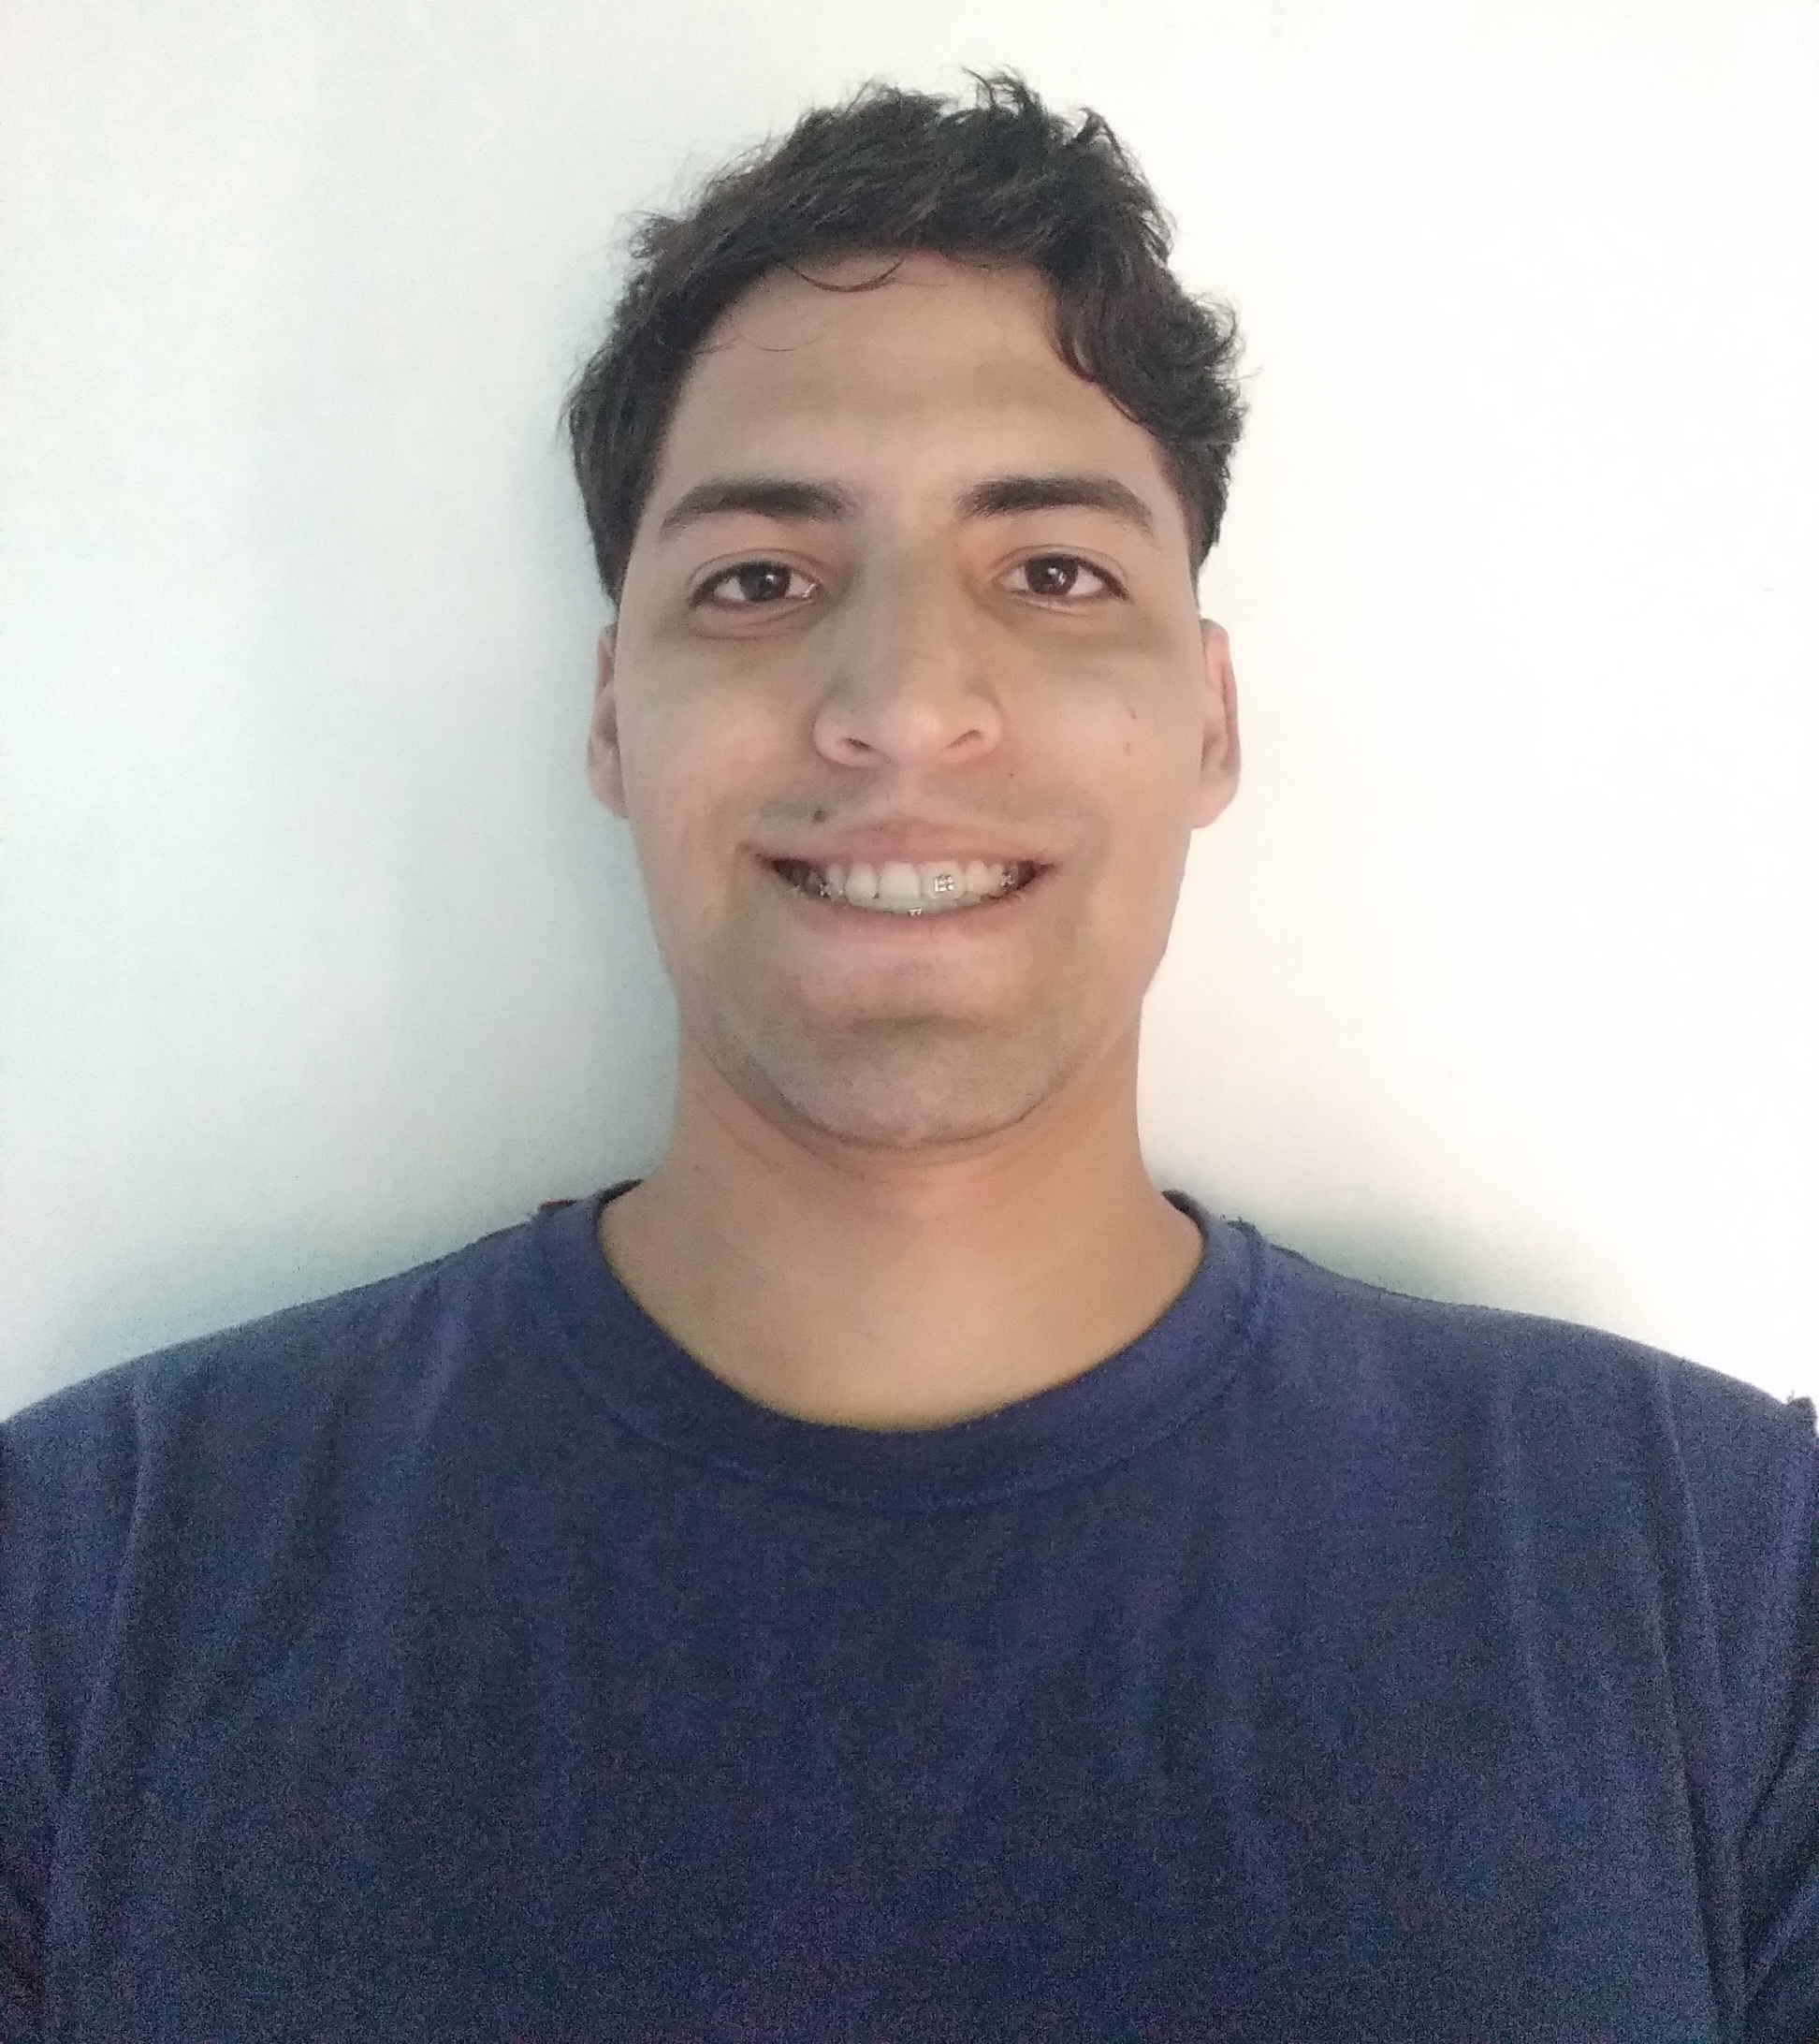
\includegraphics[width=4.2cm, height=4.5cm]{perfil.jpg}
\end{tabular}

   
\end{tabular}

\end{tabular*}

%-----------EDUCATION-----------------
%\section{~~Educación}
\vspace{10pt}
 \textcolor{NavyBlue}{ \rule[1mm]{2cm}{2mm} {\LARGE ~~Educación}}
\vspace{2pt}

  \resumeSubHeadingListStart
    \resumeSubheading
    {Ingeniería de Computación}{Sep 2019 - Presente}
      {Universidad Simón Bolívar (USB)}{Caracas, Venezuela}
    \resumeSubHeadingListEnd
    
   \resumeSubHeadingListStart
    \resumeSubheading
    {Técnico Superior Universitario - Tecnología Electrónica}{Sep 2013 - Dic 2018}
      {Universidad Simón Bolívar (USB-SL)}{Vargas, Venezuela}
    \resumeSubHeadingListEnd
	    
%\vspace{2pt}
%\section{Habilidades}
\vspace{10pt}
 \textcolor{NavyBlue}{ \rule[1mm]{2cm}{2mm} {\LARGE ~~Habilidades}}
\vspace{2pt}


\resumeSubHeadingListStart

	\resumeSubItem{Lenguajes}{~~~~~~~~~~~~~~~~~~Python, C, Assembly(PIC), MicroPython, JAVA, JavaScript, TypeScript}
	\resumeSubItem{Frameworks}{~~~~~~~~~~~~~~~Odoo(ERP/CRM), Ionic 4, Angular 9, Spring Boot}
	\resumeSubItem{Herramientas}{~~~~~~~~~~~~~GIT, PostgreSQL, MySQL, \LaTeX{}}
	\resumeSubItem{Plataformas}{~~~~~~~~~~~~~~~GNU/Linux Debian, Arduino, AWS}
	\resumeSubItem{MicroControladores}{~~~PICs, ESP8266 nodeMCU, ESP32}
	\resumeSubItem{Soft Skills}{~~~~~~~~~~~~~~~~~~IoT, HTML, CSS}
	\resumeSubItem{Protocolos}{~~~~~~~~~~~~~~~~~$I^{2}C$, SPI, UART, MQTT, Modbus TCP-IP, Modbus RTU}

\resumeSubHeadingListEnd

%\section{Experience}

\vspace{10pt}
 \textcolor{NavyBlue}{ \rule[1mm]{2cm}{2mm} {\LARGE ~~Experiencia Laboral}}
\vspace{2pt}

  \resumeSubHeadingListStart
    \resumeSubheading{Edooit C.A.}{Remoto}
    {Analista de Proyectos}{Abr 2020 - Presente}
    \resumeItemListStart
        \resumeItem{Desarrollo en odoo}
          {Creación, programación y mantenimiento de módulos en odoo versión 11 y 13 mediante Python, JavaScript, XML, PostgreSQL.}
          \resumeItem{Desarrollo en android}
          {Creación, programación y mantenimiento de APPs para android mediante Ionic v4 y Angular v9.}
          \resumeItem{Tecnologías y herramientas usadas}{GIT, XML-RPC, VScode, Pycharm, Debian, API REST, Virtual env.}
      \resumeItemListEnd
\vspace{10pt}
    \resumeSubheading
		{SkyFlot C.A.}{Presencial - Remoto}
		{Analista de Servidores}{Sep 2019 -  Abr 2020}
		\resumeItemListStart
        \resumeItem{Administración de Servidores}
          {Mantenimiento, diagnóstico preventivo y correctivo de Servidores GNU/Linux Debian y Ubuntu en AWS. Respaldo automático de DB. Gestión de permisos y acceso de usuarios. Auditoria de servicios, procesos y puertos. Gestión de memoria y procesos en segundo plano. Integración e instalación de sistemas entre Servidores.}
        \resumeItem{Soporte Técnico}
           {Gestion de incidencias sobre equipos y requerimientos de funcionalidad(programas, respaldos, reparación).}
        \resumeItem{Tecnologías y herramientas usadas}{AWS, GIT, Ubuntu, Debian, Python, Bash, DNAT/SNAT, cPanel, FreshDesk, iTop, Moodle, Apache, Nginx, PostgreSQL, MySQL, SSH, chroot.}
		\resumeItemListEnd
		
\vspace{10pt}
    \resumeSubheading
		{Mega Soft Computación C.A.}{Presencial}
		{Consultor Programador II}{Abr 2019 -  Sep 2019}
\resumeItemListStart
        \resumeItem{Programación de POS}
          {Programación de POS(Point of Sale) y afines para tecnologías orientadas a medios de pago mediante JAVA, JavaScript y TypeScript.}
          \resumeItem{Tecnologías y herramientas usadas}{JAVA, Spring Boot, Ionic v3, Angular v7, VScode, Eclipse IDE, API REST, HTML, CSS, Postman.}
      \resumeItemListEnd
\vspace{10pt}
    \resumeSubheading
		{Seguricel Telemática C.A.}{Presencial}
		{Técnico Electrónico Desarrollador Junior}{Mar 2019 -  Abr 2019}
\resumeItemListStart
        \resumeItem{Programación de Microcontroladores}
          {Desarrollo de firmware en microcontroladores para dispositivos de seguridad residencial.}
          \resumeItem{Tecnologías y herramientas usadas}{PICs (Gama media/alta), C, Arduino, ESP8266, Mplab X IDE.}
      \resumeItemListEnd
      
      \vspace{10pt}
    \resumeSubheading
		{PDVSA La Estancia S.A.}{Presencial}
		{Becario (Tiempo - parcial)}{Ene 2017 -  Ene 2018}
\resumeItemListStart
        \resumeItem{Guía}
          {Guía cultural y patrimonial de PDVSA La Estancia Sede la Floresta.}
      \resumeItemListEnd

\resumeSubHeadingListEnd

%-----------EDUCATION-----------------
%\section{~~Educación}
\vspace{10pt}
 \textcolor{NavyBlue}{ \rule[1mm]{2cm}{2mm} {\LARGE ~~Cursos}}
\vspace{2pt}

  \resumeSubHeadingListStart
  
  \resumeSubheading
    {Python 3}{Oct 2020 - No Expira}
      {SoloLearn}{{\href{https://www.sololearn.com/certificates/course/en/16131809/1073/landscape/png}{\textcolor{Blue}{credencial}}}}
      
  
    \resumeSubheading
    {Linux Tools for Developers}{Ago 2020 - No Expira}
      {Coursera}{\href{https://www.coursera.org/account/accomplishments/certificate/EYMQ32PVEM2A}{\textcolor{Blue}{credencial}}}
    \resumeSubHeadingListEnd
    \vspace{-12pt}
      \resumeSubHeadingListStart
    \resumeSubheading
    {Python Basics}{Ago 2020 - No Expira}
      {Coursera}{{\href{https://www.coursera.org/account/accomplishments/certificate/4MSUPEDPGEEB}{\textcolor{Blue}{credencial}}}}
      
      \resumeSubheading
    {Java Avanzado 2}{Jul 2020 - No Expira}
      {LinkedIn}{}
      
      \resumeSubheading
    {JavaScript esencial}{Jul 2020 - No Expira}
      {LinkedIn}{}
      
    \resumeSubheading
    {Linux for Developers}{Jun 2020 - No Expira}
      {Coursera}{{\href{https://www.coursera.org/account/accomplishments/certificate/6Z8B83NFBSZE}{\textcolor{Blue}{credencial}}}}
    \resumeSubheading
    {jQuery Tutorial}{Jun 2020 - No Expira}
      {SoloLearn}{{\href{https://www.sololearn.com/Certificate/1082-16131809/pdf/}{\textcolor{Blue}{credencial}}}}
      \resumeSubheading
    {Open Source Software Development Methods}{Abr 2020 - No Expira}
      {Coursera}{{\href{https://www.coursera.org/account/accomplishments/certificate/LPWWCHWCE9N9}{\textcolor{Blue}{credencial}}}}
           \resumeSubheading
    {Instalaciones Eléctricas Residenciales}{Nov 2015 - No Expira}
      {Universidad Simón Bolívar}{}
    \resumeSubHeadingListEnd
    


%-----------PROJECTS-----------------
%\vspace{-5pt}
%\section{Projects}


%DEScomentar despues
%\vspace{10pt}
% \textcolor{NavyBlue}{ \rule[1mm]{2cm}{2mm} {\LARGE ~~Proyectos}}
%\vspace{2pt}

%\resumeSubHeadingListStart
%\resumeSubItem{Vison - multimedia search engine (NLP, Search Engine, Web Crawlers, Multimedia Processing)}{(Work in progress) Research oriented, open source, search engine for bringing reverse multimedia search to small \& mid scale enterprises. Tech: Python, NodeJS, Intel OpenVino Toolkit, Selenium, TensorFlow (October '18)}
%\vspace{2pt}
%\resumeSubItem{Reinforcement Learning based Traffic Control System (Reinforcement Learning, Computer Vision)}{AI model to resolve city traffic around 50\%
%faster. Tech: Python, Alibaba Cloud, Raspberry Pi, Arduino, SUMO \& OpenCV. (August '18)}
%\vspace{2pt}
%\resumeSubItem{Panorama from Satellite Imagery using Distributed Computing (Distributed Computing, Image Processing)}{Images clicked using drones, provided by ISRO were stitched together using distributed public compute nodes, effectively bringing down processing time exponentially. Tech: PHP, C++, Java, Python (March '18)}
%\vspace{2pt}
%\resumeSubItem{Drag-n-drop machine learning learning environment (Web Development, Machine Learning)}{Scratch like tool for implementing machine learning pipelines along with built in tutorial for each concept. Tech: Python, JavaScript (September '18)}
%\vspace{2pt}
%\resumeSubItem{Search Engine and Social Network(Web Development, Web Crawler, Search)}{Created from scratch a social network and a search engine based on the idea of integrating Facebook and Google. The launched website was among top 1000 websites in India during 2012-2013. Tech: PHP, MySQL, HTML, CSS, WebSockets, JavaScript, RSS, XML ( May '12)}
%\resumeSubHeadingListEnd
%\vspace{-5pt}
%\section{Publications}
%\vspace{10pt}
% \textcolor{NavyBlue}{ \rule[1mm]{2cm}{2mm} {\LARGE ~~Publicaciones}}
%\vspace{2pt}
%\resumeSubHeadingListStart
%\resumeSubItem{Book: Deep Learning on Web (Web Development, Deep Learning)}{Work in Progress book to be published by Packt Publishing in late 2019. Tech: Django, Python, AWS, GCP, Azure (November '18)}
%\vspace{2pt}
%\resumeSubItem{Book: Deep Learning on Mobile Devices (Flutter App Development, Deep Learning)}{Work in Progress book to be published by Packt Publishing in late 2019. Tech: Flutter, Android, Firebase, TensorFlow, Python, Dart (December '18)}
%\resumeSubHeadingListEnd
%\vspace{-5pt}



%-----------Awards-----------------
%\section{Honors and Awards}
\vspace{10pt}
 \textcolor{NavyBlue}{ \rule[1mm]{2cm}{2mm} {\LARGE ~~Premios y Reconocimientos}}
\vspace{2pt}
\begin{description}[font=$\bullet$]
\item {\textbf{Mención especial de "Excepcionalmente Bueno" en presentación de informe de pasantía:}}\\
 {Ingeniería inversa del módulo Esclavo del protocolo de comunicación Modbus TCP-IP y del Gestor de los \\módulos de comunicación implementados en la NET-DAS v2.0 para PDVSA INTEVEP, S.A. - (Oct, 2018)}\\
 \vspace{4pt}
 {{\href{https://drive.google.com/file/d/1bHQlD1dOGpO19o5fX3Z03ocKmDDeeF34/view}{\textcolor{Blue}{Enlace del informe}}}}
 %

\end{description}


\vspace{-5pt}
%\section{Volunteer Experience}
\vspace{10pt}
 \textcolor{NavyBlue}{ \rule[1mm]{2cm}{2mm} {\LARGE ~~Experiencia de Voluntariado}}
\vspace{2pt}
  \resumeSubHeadingListStart
	\resumeSubheading
    {GuardaBosques universitarios de la Universidad Simón Bolívar}{Sartenejas, Venezuela}
    {Incitación a la participación de los ciudadanos para el cuidado de la biodiversidad.}{Jul 2017 - Mar 2018}
\resumeSubHeadingListEnd

\end{document}

